%% MiPaper.tex
%% Paper: Empirical Analysis of the Impact of MVP, MVVM and MVI Patterns
%% on Android Code Maintainability through Repository Mining
%% Author: Daniel Solano Avila - Universidad Nacional de Costa Rica

\documentclass[conference]{IEEEtran}

\usepackage[utf8]{inputenc}
\usepackage{cite}
\usepackage{url}
\usepackage{graphicx}
\usepackage{multirow}
\usepackage{booktabs}

\graphicspath{{figures/}}
\hyphenation{main-tain-a-bil-i-ty ar-chi-tec-ture re-pos-i-to-ries pre-sen-ta-tion}

\begin{document}

% -------------------------------------------------------
% TITLE
% -------------------------------------------------------
\title{Empirical Analysis of the Impact of MVP, MVVM and MVI Patterns\\
on Android Code Maintainability\\
through Repository Mining}

\author{\IEEEauthorblockN{Daniel Solano \'Avila}
\IEEEauthorblockA{School of Systems Engineering\\
Universidad Nacional de Costa Rica\\
Email: daniel.solano.avila@est.una.ac.cr}}

\maketitle

% -------------------------------------------------------
% ABSTRACT  (finalized once results are in)
% -------------------------------------------------------
\begin{abstract}
The Android ecosystem has evolved from monolithic \texttt{Activity}/\texttt{Fragment}
designs toward separation-of-concerns patterns: Model-View-Presenter (MVP),
Model-View-ViewModel (MVVM) and Model-View-Intent (MVI). Despite their growing
adoption, quantitative evidence comparing their effect on maintainability is scarce.
This paper reports an empirical study that mines open-source Android applications from
GitHub and measures, with a single uniform Kotlin/Java static-analysis toolchain, the
structural quality of their presentation layer (coupling CBO, cohesion LCOM, complexity
WMC) together with a history-based change-proneness signal. Metrics are computed for a
curated corpus of code-confirmed MVP, MVVM and MVI applications and compared with
non-parametric tests (Kruskal--Wallis, pairwise Mann--Whitney with Holm correction) and
Cliff's $\delta$ effect sizes. Our extractor is validated against the established CK tool
(Spearman $\rho=0.83$ for CBO and $0.85$ for WMC over $1{,}204$ Java classes).
Across 28 code-confirmed applications, MVP shows the lowest \emph{median}
presentation-layer coupling (large effect sizes versus MVVM and MVI) while MVVM
and MVI are structurally indistinguishable in coupling; MVI attains the simplest individual
classes (lowest WMC) at the cost of the lowest cohesion, whereas MVVM concentrates
logic in more complex ViewModels. No pattern shows significantly different
change-proneness. The study provides objective evidence to guide architectural
selection in medium-scale Android development and a fully reproducible
mining-and-analysis pipeline.
\end{abstract}

\begin{IEEEkeywords}
architectural patterns, Android, MVP, MVVM, MVI, maintainability, code metrics,
mining software repositories, change-proneness.
\end{IEEEkeywords}

% -------------------------------------------------------
% SECTION 1: INTRODUCTION
% -------------------------------------------------------
\section{Introduction} \label{sec:Introduction}

Android application development has undergone a significant transformation
since the early days of the ecosystem. In its initial stages, the platform
encouraged a model where \texttt{Activity} and \texttt{Fragment} classes
concentrated both business logic and visual presentation, giving rise to
what are known as \textit{God Objects} or \textit{Massive View Controllers}
\cite{Vijaywargi:2024}. While functional for simple applications, this approach
presented serious limitations in scalability, testability, and maintenance
as projects grew in complexity.

To address these shortcomings, Google and the developer community promoted
the adoption of separation-of-concerns patterns. The Model-View-Presenter
(MVP) pattern emerged as one of the first widely adopted alternatives.
Later, with the introduction of Android \textit{Architecture Components},
the Model-View-ViewModel (MVVM) pattern gained considerable popularity
thanks to its native integration with tools such as \texttt{LiveData} and
\texttt{ViewModel} \cite{Pradana:2025}.

With the arrival of \textit{Jetpack Compose}, a declarative UI toolkit,
architectures based on unidirectional data flow and immutable state have
emerged strongly. The Model-View-Intent (MVI) pattern presents itself as
a more predictable solution to the accidental recomposition issues that
MVVM can suffer under the declarative paradigm \cite{Vijaywargi:2024}.

\subsection{Problem and Justification}

Despite the existence of many theoretical debates about the advantages and
disadvantages of each pattern, quantitative evidence remains scarce. The
lack of consensus and empirical evidence makes it difficult for development
teams to choose the right architecture for their projects. A poor choice
generates high technical debt, reflected in metrics such as high Coupling
Between Objects (CBO) and low cohesion (high LCOM), which complicate
long-term maintenance \cite{Filo:2024,ChidamberKemerer:1994}.

An objective empirical analysis is needed to compare these architectures
based on concrete, measurable metrics. Extracting real data through Mining
Software Repositories (MSR) techniques on GitHub allows an objective evaluation
of which architecture better contains coupling, preserves cohesion, and limits
the change-proneness of the presentation layer, thus going beyond purely
opinion-based debates \cite{Kalliamvakou:2014}.

\subsection{Objective}

To empirically analyze the impact of the MVP, MVVM, and MVI architectural
patterns on the maintainability of medium-scale Android applications, through
the extraction and comparison of presentation-layer static code metrics
(WMC, CBO, LCOM) and a history-based change-proneness signal obtained from
open-source projects on GitHub.

\subsection{Paper Outline}

The remainder of this document is organized as follows: Section~\ref{sec:RQ}
presents the research questions. Section~\ref{sec:Related} reviews related work.
Section~\ref{sec:Background} describes the theoretical background.
Section~\ref{sec:Method} details the repository-mining and static-analysis
methodology. Section~\ref{sec:Results} reports the results, and
Section~\ref{sec:Discussion} interprets them and contrasts them with related
work. Section~\ref{sec:Threats} discusses threats to validity, and
Section~\ref{sec:Conclusions} presents conclusions and future work.

% -------------------------------------------------------
% SECTION 2: RESEARCH QUESTIONS
% -------------------------------------------------------
\section{Research Questions} \label{sec:RQ}

Based on the identified problem, this study poses the following research
questions:

\begin{description}
  \item[\textbf{RQ1:}] Which architectural pattern (MVP, MVVM, or MVI)
  produces the lowest coupling (CBO), the highest cohesion (lowest LCOM)
  and the lowest complexity (WMC) in the presentation layer of Android
  applications?
  \item[\textbf{RQ2:}] Are there significant differences in the
  \textit{change-proneness} of the presentation layer (how frequently its
  code is modified over the project history) among applications implemented
  under the MVP, MVVM and MVI patterns?
\end{description}

The first question targets the \emph{internal structural quality} of the
presentation layer at a single point in time; the second targets its
\emph{evolution} over time, a complementary and directly mineable proxy of
maintainability in practice \cite{Khomh:2009}. Runtime performance, considered
in earlier proposals, is intentionally left out because it cannot be obtained
from repository mining without executing each application; it is revisited as
future work (Section~\ref{sec:Conclusions}).

% -------------------------------------------------------
% SECTION 3: RELATED WORK
% -------------------------------------------------------
\section{Related Work} \label{sec:Related}

Vijaywargi and Boddapati \cite{Vijaywargi:2024} performed a qualitative
comparison of MVP, MVVM and MVI in modern Android development, concluding that
MVI offers greater predictability in state management at the cost of a steeper
learning curve. Their analysis, however, did not include quantitative
code-quality metrics, a gap this study addresses.

Pradana et al. \cite{Pradana:2025} conducted a comparative performance analysis
of MVVM and MVP on a single Android dashboard system, measuring response time
and memory usage and reporting statistically significant differences in memory
consumption under load. Because the study was limited to one controlled project,
its generalization is restricted; we instead mine many real projects, trading
runtime measurement for breadth and external validity.

Kalliamvakou et al. \cite{Kalliamvakou:2014} documented the promises and perils
of mining GitHub, warning about biases such as the prevalence of personal or
inactive repositories and the difficulty of inferring causality from
observational data. These warnings directly shaped our inclusion/exclusion
criteria and manual validation step (Section~\ref{sec:Method}).

The object-oriented metrics we adopt originate in the suite of Chidamber and
Kemerer \cite{ChidamberKemerer:1994} (CBO, WMC and the original LCOM), later
refined by Henderson-Sellers \cite{HendersonSellers:1996}, whose normalized
LCOM-HS we use. Fil\'o et al. \cite{Filo:2024} derived empirical thresholds for
these metrics from a large corpus of open-source Java projects; we use those
thresholds as comparison baselines. To compute the metrics consistently across
Kotlin and Java we build on the same definitions implemented by the widely used
CK tool \cite{Aniche:2015}, against which we validate our extractor.

Finally, change-proneness, the frequency with which a class or file is modified,
is a well-established external indicator of maintainability: Khomh et al.
\cite{Khomh:2009} showed that structurally degraded classes are significantly
more change-prone. We mine this signal from version history as our second,
evolution-oriented response variable.

% -------------------------------------------------------
% SECTION 4: BACKGROUND
% -------------------------------------------------------
\section{Background} \label{sec:Background}

\subsection{Architectural Patterns in Android}

Architectural patterns define how responsibilities are separated among the
components of an application. The three patterns central to this study are the
following.

\textbf{MVP (Model-View-Presenter)} separates presentation logic into a
\textit{Presenter} that mediates between the data model and a passive view, so
that the view delegates every logical decision to the presenter.

\textbf{MVVM (Model-View-ViewModel)} introduces a \textit{ViewModel} that exposes
observable data streams (e.g., \texttt{LiveData} or \texttt{StateFlow}); the view
subscribes to these streams, which removes the direct view--logic reference. It
is the pattern officially recommended by Google for projects built on the
Architecture Components.

\textbf{MVI (Model-View-Intent)} implements a strictly unidirectional data flow:
the UI state is immutable and is updated only through \textit{intents} that
produce a new state, typically via a \texttt{reduce} function. It is particularly
well suited to Jetpack Compose.

A key observation, confirmed during this study, is that on Android MVI is almost
always \emph{built on top of} the MVVM infrastructure (a \texttt{ViewModel}
holding an immutable \texttt{StateFlow}). The patterns therefore form a
progression rather than disjoint categories, which has direct consequences for
their automated classification (Section~\ref{sec:Method}).

\subsection{Code Quality Metrics}

To assess structural maintainability we use the following object-oriented
metrics \cite{ChidamberKemerer:1994,HendersonSellers:1996,Filo:2024}.

\textbf{WMC (Weighted Methods per Class)} is the sum of the cyclomatic complexity
of all methods of a class; higher values indicate greater complexity and
maintenance effort.

\textbf{CBO (Coupling Between Objects)} is the number of other classes a class is
coupled to; high CBO hinders unit testing and reuse.

\textbf{LCOM (Lack of Cohesion in Methods)} is the degree to which the methods of
a class fail to share instance attributes. We use the normalized
Henderson-Sellers variant (LCOM-HS); higher values indicate lower cohesion.

\textbf{SLOC (Source Lines of Code)} and \textbf{NOM (Number of Methods)} are
size measures used for normalization and characterization.

\subsection{Mining Software Repositories}

Mining Software Repositories (MSR) extracts and analyzes data from version
control systems and other digital sources to obtain empirical knowledge about
software development \cite{Kalliamvakou:2014}. In this study GitHub is the
primary data source, and rigorous selection criteria are applied to mitigate the
biases identified in the literature.

% -------------------------------------------------------
% SECTION 5: METHODOLOGY
% -------------------------------------------------------
\section{Methodology} \label{sec:Method}

The study follows the guidelines for empirical experimentation in software
engineering \cite{Wohlin:2012}. The whole process is implemented as a
reproducible pipeline of Python and Java scripts; all data and scripts are
released with the paper.

\subsection{Corpus Selection and Classification}
GitHub's search API is queried for native Android repositories declaring an MVP,
MVVM or MVI architecture. Inclusion criteria require a native Android language
(Kotlin/Java), an open-source license, at least six months of history and
activity within the last twelve months. Repositories are excluded if they are
forks, archived, tutorial/sample collections, or \emph{consumable libraries or
frameworks} (detected through topics, publishing plugins and a manually curated
list); the latter is essential because the most popular ``MVP/MVI'' repositories
are architecture libraries rather than applications. Each candidate is cloned
and its pattern is \emph{confirmed from code signals} (presence of
\texttt{Presenter} classes, \texttt{ViewModel}s with observable state, or
unidirectional-flow markers such as sealed intents and \texttt{reduce}), not from
its README. Because MVI is implemented on top of MVVM, a precedence rule assigns
MVI when its distinctive markers are present. From roughly $7{,}000$ candidate
repositories returned by the queries, $232$ satisfied the automated eligibility
filters; after pattern confirmation and a manual audit removing libraries and
misclassified projects, the final corpus comprised \textbf{30 applications}
(MVVM~$=12$, MVI~$=12$, MVP~$=6$). Genuine MVP applications proved very scarce:
every highly starred ``MVP'' repository was in fact an architecture library, so
the MVP group is necessarily small and low in popularity. Table~\ref{tab:corpus}
lists the most popular application of each pattern as an illustration of the
corpus and of this popularity gap.

\begin{table}[!t]
\centering
\caption{Representative applications in the corpus (highest-starred per pattern;
the full list of 28 is in the released data)}
\label{tab:corpus}
\resizebox{\columnwidth}{!}{%
\begin{tabular}{|l|l|r|l|}
\hline
\textbf{Pattern} & \textbf{Application} & \textbf{Stars} & \textbf{Lang.} \\ \hline
\multirow{3}{*}{MVP}  & JsonChao/Awesome-WanAndroid      & 2{,}719 & Java   \\
                      & RznNike/EyeHealthManager         & 6       & Kotlin \\
                      & siempredelao/Distance-From-Me     & 4       & Kotlin \\ \hline
\multirow{3}{*}{MVVM} & TeamAmaze/AmazeFileManager        & 6{,}212 & Kotlin \\
                      & youlookwhat/CloudReader           & 5{,}011 & Java   \\
                      & tanujnotes/Olauncher              & 3{,}602 & Kotlin \\ \hline
\multirow{3}{*}{MVI}  & v1tzor/TimePlanner                & 634     & Kotlin \\
                      & SkyD666/Rays-Android              & 326     & Kotlin \\
                      & SkyD666/Raca-Android              & 117     & Kotlin \\ \hline
\end{tabular}}
\\[2pt] \footnotesize{The disparity in popularity between MVP and the other two
groups is itself a finding: genuine, highly starred MVP \emph{applications} are
scarce because most popular ``MVP'' repositories are architecture libraries.}
\end{table}


\subsection{Static Metric Extraction}
A single tree-sitter-based extractor parses both Kotlin and Java and computes,
per class, SLOC, NOM, WMC, CBO and LCOM-HS, using uniform definitions across
languages. Only \emph{presentation-layer logic holders} (Presenters, ViewModels,
stores/reducers, or classes extending a ViewModel base) with at least one method
are aggregated, so that the comparison is equitable across patterns and not
diluted by empty marker or pure-data classes. Per-class metrics are aggregated to
\emph{per-repository medians} to avoid pseudo-replication (classes within a repository
are not independent). Two MVI projects whose state holders use a non-standard
naming convention contributed no logic holder and were dropped, leaving
$28$ applications for analysis (MVVM~$=12$, MVI~$=10$, MVP~$=6$).

\subsection{Extractor Validation}
To establish construct validity, the extractor is run alongside CK
\cite{Aniche:2015} on the Java subset of the corpus and the two are compared with
Spearman correlation over $1{,}204$ matched Java classes. Agreement is strong for
CBO ($\rho=0.83$) and WMC ($\rho=0.85$) and moderate for LCOM ($\rho=0.58$,
expected because CK implements a different LCOM variant), confirming that the
custom extractor measures the same constructs as an established tool.

\subsection{Change-Proneness}
For RQ2, the git history of each presentation-layer file is mined to obtain the
number of commits that touched it and the churn (lines added plus deleted),
normalized respectively by the repository's active lifetime and by file size, and
aggregated to per-repository medians.

\subsection{Statistical Procedure}
Because the samples are independent (different repositories per pattern), the
omnibus Kruskal--Wallis test is applied to each metric, followed by pairwise
Mann--Whitney $U$ tests with Holm correction and Cliff's $\delta$ effect sizes
($\alpha=0.05$). This corrects earlier proposals that suggested the Wilcoxon
signed-rank test, which assumes paired data.

% -------------------------------------------------------
% SECTION 6: RESULTS  (auto-filled from generated tables/figures)
% -------------------------------------------------------
\section{Results and Analysis} \label{sec:Results}

The analysis covers the $28$ applications with measurable presentation-layer
logic holders. Table~\ref{tab:summary} gives a one-line summary of the headline
findings; Table~\ref{tab:desc_rq1} summarizes the per-repository median metrics by
pattern and Table~\ref{tab:tests_rq1} reports the statistical tests.

\begin{table}[!t]
\centering
\caption{One-line summary of findings by research question}
\label{tab:summary}
\begin{tabular}{|c|p{6.7cm}|}
\hline
\textbf{RQ} & \textbf{Key finding} \\ \hline
RQ1 & MVP shows the lowest \emph{median} coupling (large effect sizes vs.\ MVVM
and MVI, though the omnibus test is borderline). MVVM and MVI are indistinguishable
in coupling and differ only in \emph{where} they place logic: MVVM concentrates it
in fewer, more complex ViewModels (high WMC), MVI spreads it across many small but
less cohesive classes. \\ \hline
RQ2 & No significant difference in change-proneness (commits per month or churn per
SLOC) across patterns; presentation-layer evolution appears driven by product and
team factors rather than the architectural pattern. \\ \hline
\end{tabular}
\end{table}

\begin{table}[!t]
\centering
\caption{Presentation-layer structural metrics by pattern (per-repository medians)}
\label{tab:desc_rq1}
\resizebox{\columnwidth}{!}{%
\begin{tabular}{|l|l|r|r|r|r|r|r|}
\hline
\textbf{Metric} & \textbf{Pattern} & \textbf{n} & \textbf{Median} & \textbf{Mean} & \textbf{IQR} & \textbf{Min} & \textbf{Max} \\ \hline
\multirow{3}{*}{CBO}  & MVP  & 6  & 6.50  & 6.67  & 4.00  & 3.00 & 11.00 \\
                      & MVVM & 12 & 10.50 & 12.25 & 6.00  & 5.50 & 22.00 \\
                      & MVI  & 10 & 11.00 & 11.45 & 6.88  & 3.00 & 19.50 \\ \hline
\multirow{3}{*}{LCOM} & MVP  & 6  & 0.85  & 0.90  & 0.18  & 0.64 & 1.35  \\
                      & MVVM & 11 & 0.91  & 0.98  & 0.10  & 0.82 & 1.67  \\
                      & MVI  & 9  & 0.97  & 1.02  & 0.07  & 0.66 & 1.50  \\ \hline
\multirow{3}{*}{WMC}  & MVP  & 6  & 5.00  & 6.00  & 5.00  & 3.00 & 11.00 \\
                      & MVVM & 12 & 12.50 & 17.58 & 11.88 & 1.00 & 84.00 \\
                      & MVI  & 10 & 4.00  & 7.80  & 8.13  & 2.00 & 21.00 \\ \hline
\end{tabular}}
\\[2pt] \footnotesize{Higher CBO, LCOM-HS and WMC all indicate worse
maintainability. LCOM is defined for fewer repositories because state holders
with a single method have undefined cohesion.}
\end{table}


\subsection{RQ1 -- Presentation-Layer Structure}

\textbf{Coupling (CBO).} MVP exhibits the lowest \emph{median} coupling ($6.5$),
below MVVM ($10.5$) and MVI ($11.0$); see Fig.~\ref{fig:rq1}. The Kruskal--Wallis
test is borderline ($H=5.36$, $p=0.069$) and, although Holm-corrected pairwise
$p$-values do not cross $\alpha=0.05$ given the small samples, the effect sizes are
\emph{large} for MVP versus MVVM (Cliff's $\delta=-0.67$) and MVP versus MVI
($\delta=-0.55$). In contrast, MVVM and MVI are statistically indistinguishable
($\delta=0.10$, negligible), which is consistent with MVI being built upon the
MVVM infrastructure on Android.

\textbf{Cohesion (LCOM-HS).} A consistent monotonic trend appears: cohesion
degrades from MVP ($0.85$) through MVVM ($0.91$) to MVI ($0.97$, i.e., the least
cohesive), with a large effect for MVP versus MVI ($\delta=-0.48$) and a medium
effect for MVVM versus MVI ($\delta=-0.36$). The many small, interlinked
state/intent/reducer classes of MVI appear to spread responsibilities at the cost
of cohesion. LCOM is defined for fewer repositories (MVVM~$n=11$, MVI~$n=9$)
because single-method state holders have undefined cohesion and are therefore
excluded from this metric only.

\textbf{Complexity (WMC).} The picture inverts: MVVM concentrates logic in
comparatively complex ViewModels (median WMC $12.5$), whereas both MVP ($5.0$) and
MVI ($4.0$) keep individual presentation classes simple (MVP vs.\ MVVM
$\delta=-0.46$, medium). MVI thus trades higher coupling and lower cohesion for
lower per-class complexity, distributing behaviour across more classes.

\begin{table}[!t]
\centering
\caption{RQ1 -- Kruskal-Wallis and pairwise Mann-Whitney (Holm)}
\label{tab:tests_rq1}
\resizebox{\columnwidth}{!}{%
\begin{tabular}{|l|l|r|r|r|l|}
\hline
\textbf{Metric} & \textbf{Pair} & \textbf{$p_{KW}$} & \textbf{$p_{Holm}$} & \textbf{$\delta$} & \textbf{Effect} \\ \hline
CBO & MVP vs MVVM & 0.069 & 0.080 & -0.67 & large \\ \hline
CBO & MVP vs MVI & 0.069 & 0.164 & -0.55 & large \\ \hline
CBO & MVVM vs MVI & 0.069 & 0.715 & 0.10 & negligible \\ \hline
LCOM & MVP vs MVVM & 0.179 & 0.421 & -0.30 & small \\ \hline
LCOM & MVP vs MVI & 0.179 & 0.421 & -0.48 & large \\ \hline
LCOM & MVVM vs MVI & 0.179 & 0.421 & -0.36 & medium \\ \hline
WMC & MVP vs MVVM & 0.273 & 0.398 & -0.46 & medium \\ \hline
WMC & MVP vs MVI & 0.273 & 0.783 & 0.10 & negligible \\ \hline
WMC & MVVM vs MVI & 0.273 & 0.493 & 0.30 & small \\ \hline
\end{tabular}}
\\[2pt] \footnotesize{* significant at $\alpha=0.05$ after Holm correction.}
\end{table}

\begin{figure}[!t]
\centering
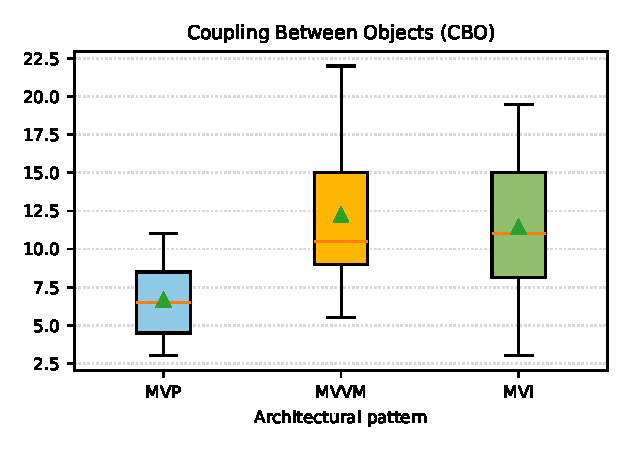
\includegraphics[width=0.72\columnwidth]{box_CBO.pdf}\\
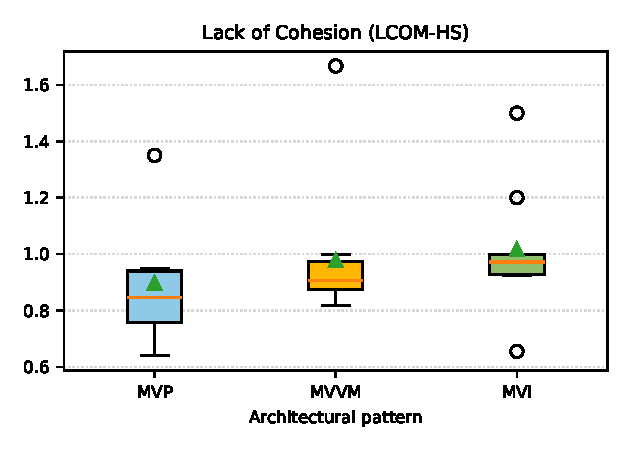
\includegraphics[width=0.72\columnwidth]{box_LCOM.pdf}\\
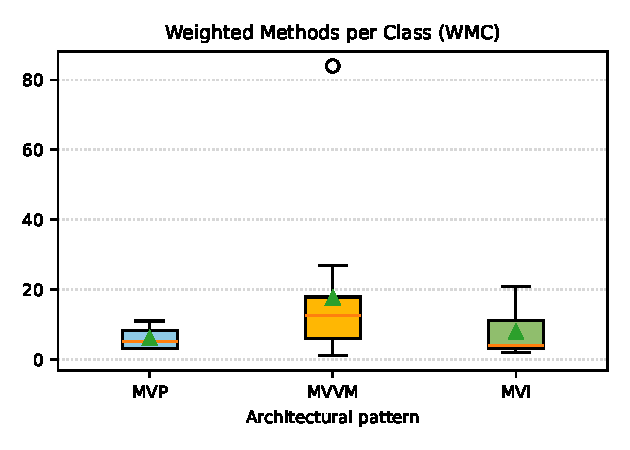
\includegraphics[width=0.72\columnwidth]{box_WMC.pdf}
\caption{Presentation-layer coupling (CBO, top), cohesion (LCOM-HS, middle) and
complexity (WMC, bottom) by architectural pattern (per-repository medians). For
LCOM-HS and WMC, higher is worse; the threshold from Fil\'o et al.\
\cite{Filo:2024} is drawn as a reference where applicable.}
\label{fig:rq1}
\end{figure}

\subsection{RQ2 -- Change-Proneness}

No statistically significant differences were found in either change frequency
(commits per month) or churn per SLOC of the presentation layer (Kruskal--Wallis
$p=0.78$ and $p=0.54$ respectively), and all pairwise effect sizes are negligible
to small (Table~\ref{tab:tests_rq2}, Fig.~\ref{fig:rq2}). Within this corpus, the
architectural pattern does not materially affect how frequently the presentation
layer is modified over the project history; evolution effort appears to be driven
by factors other than the chosen pattern.

\begin{table}[!t]
\centering
\caption{RQ2 -- Change-proneness tests}
\label{tab:tests_rq2}
\resizebox{\columnwidth}{!}{%
\begin{tabular}{|l|l|r|r|r|l|}
\hline
\textbf{Metric} & \textbf{Pair} & \textbf{$p_{KW}$} & \textbf{$p_{Holm}$} & \textbf{$\delta$} & \textbf{Effect} \\ \hline
Commits/month & MVP vs MVVM & 0.776 & 1.000 & -0.11 & negligible \\ \hline
Commits/month & MVP vs MVI & 0.776 & 1.000 & -0.20 & small \\ \hline
Commits/month & MVVM vs MVI & 0.776 & 1.000 & -0.12 & negligible \\ \hline
Churn/SLOC & MVP vs MVVM & 0.544 & 1.000 & -0.08 & negligible \\ \hline
Churn/SLOC & MVP vs MVI & 0.544 & 1.000 & 0.17 & small \\ \hline
Churn/SLOC & MVVM vs MVI & 0.544 & 0.829 & 0.28 & small \\ \hline
\end{tabular}}
\\[2pt] \footnotesize{* significant at $\alpha=0.05$ after Holm correction.}
\end{table}

\begin{figure}[!t]
\centering
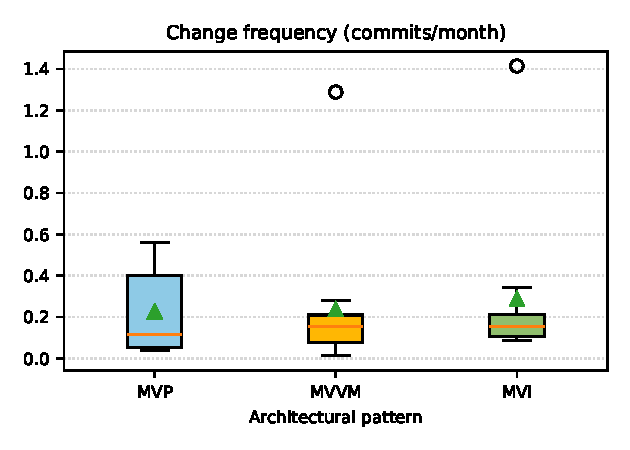
\includegraphics[width=0.72\columnwidth]{box_median_commits_per_month.pdf}\\
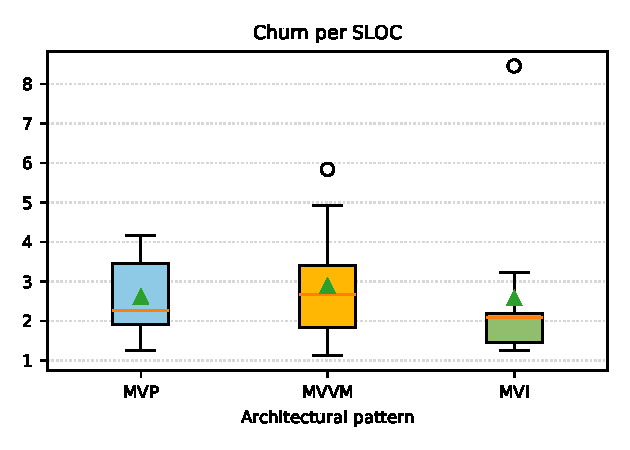
\includegraphics[width=0.72\columnwidth]{box_median_churn_per_sloc.pdf}
\caption{Change-proneness of the presentation layer by architectural pattern
(per-repository medians): change frequency in commits per month (top) and churn
per SLOC (bottom). The distributions overlap heavily across patterns.}
\label{fig:rq2}
\end{figure}

% -------------------------------------------------------
% SECTION 7: DISCUSSION
% -------------------------------------------------------
\section{Discussion} \label{sec:Discussion}

Taken together, the two research questions paint a coherent and somewhat
counter-intuitive picture of how the choice of architectural pattern relates to
the maintainability of the Android presentation layer.

\textbf{On RQ1, structure is shaped less by the pattern label than by where each
pattern places its logic.} The clearest structural separation is between MVP and
the two modern patterns: MVP exhibits substantially lower \emph{median} coupling,
with large effect sizes, even though the omnibus test stays just above
significance because the groups are small. MVVM and MVI, in contrast, are statistically
indistinguishable in coupling. This is consistent with the observation,
confirmed during corpus construction, that on Android MVI is typically
\emph{implemented on top of} MVVM (a \texttt{ViewModel} that exposes an immutable
\texttt{StateFlow}); the two are points on a continuum rather than competing
families. Their real difference is one of \emph{distribution} of behaviour:
MVVM concentrates logic in fewer but more complex ViewModels (high WMC), whereas
MVI spreads it across many small state, intent and reducer classes that lower
per-class complexity at the cost of higher coupling and lower cohesion. In other
words, MVI does not remove complexity, it relocates it from inside a class to the
relationships between classes.

\textbf{On RQ2, the pattern does not explain how the presentation layer evolves.}
Neither change frequency nor churn differs across patterns. Within this corpus,
how often presentation code is rewritten appears to be governed by product and
team factors (domain, feature pressure, contributor turnover) rather than by the
architectural style, echoing the warning of Kalliamvakou et al.
\cite{Kalliamvakou:2014} that observational repository data captures many
confounds at once.

These results refine, rather than contradict, prior work. The qualitative
comparison of Vijaywargi and Boddapati \cite{Vijaywargi:2024} credits MVI with
greater state predictability; our quantitative view adds a caveat, namely that
this predictability comes with measurably lower cohesion and higher coupling in
the state-holding classes, so ``cleaner'' is not the same as ``more cohesive.''
Pradana et al.\ \cite{Pradana:2025} found runtime memory differences between MVVM
and MVP on a single controlled project; our cross-project structural evidence is
orthogonal to that finding and shows that, structurally, MVVM and MVI are far
closer to each other than either is to MVP.

\textbf{Implications for practitioners.} For teams already on the Architecture
Components stack, the decision between MVVM and MVI is unlikely to be settled by
raw structural metrics, since the two are nearly equivalent in coupling; it
should instead be driven by considerations such as state-management
predictability, testing strategy and team familiarity. The single most actionable
signal we observe is that ViewModel complexity (WMC) can grow large under MVVM, so
teams that deliberately keep ViewModels small recover most of the structural
benefit that MVI obtains by construction, without fragmenting the codebase.

% -------------------------------------------------------
% SECTION 8: THREATS TO VALIDITY
% -------------------------------------------------------
\section{Threats to Validity} \label{sec:Threats}

\textbf{Construct validity.} CBO is computed as a syntactic coupling proxy
(distinct referenced types) rather than through full type resolution; the strong
correlation with CK ($\rho=0.83$) mitigates this concern. LCOM has several
incompatible definitions in the literature; we fix and report the
Henderson-Sellers variant.

\textbf{Internal validity.} Pattern membership is inferred from code signals and
may misclassify hybrid designs; the MVI/MVVM overlap is intrinsic to Android and
is handled by an explicit precedence rule and a manual audit. Aggregating to
per-repository medians prevents large repositories from dominating the analysis.
Because the available MVP applications are systematically smaller and less popular
than the MVVM/MVI ones, MVP's lower coupling and complexity may be partly a
\emph{size} effect rather than a pure pattern effect; the MVP results should
therefore be read as indicative rather than conclusive.

\textbf{External validity.} The corpus is biased toward popular, well-maintained
open-source projects, which are not representative of all Android software
\cite{Kalliamvakou:2014}. Genuine MVP applications are scarce and small, yielding
an unbalanced and limited MVP sample; results for that pattern must be read with
caution.

\textbf{Conclusion validity.} Group sizes are modest, especially for MVP; we
therefore report effect sizes (Cliff's $\delta$) alongside $p$-values and apply
multiple-comparison correction.

% -------------------------------------------------------
% SECTION 8: CONCLUSIONS
% -------------------------------------------------------
\section{Conclusions and Future Work} \label{sec:Conclusions}

This work presented a reproducible empirical study comparing the impact of the
MVP, MVVM and MVI architectural patterns on the maintainability of the
presentation layer of real Android applications, combining repository mining,
uniform Kotlin/Java static analysis and version-history change-proneness over a
code-confirmed corpus of 28 applications.

The study answers its two research questions directly. \textbf{RQ1:} MVP shows
the lowest \emph{median} presentation-layer coupling (large effect sizes, though
the omnibus test is borderline), but MVVM and MVI are
structurally indistinguishable in coupling and differ only in how they distribute
logic, MVVM in fewer complex ViewModels and MVI across many simpler but less
cohesive classes. \textbf{RQ2:} the architectural pattern does not explain the
change-proneness of the presentation layer; no significant differences arise in
either change frequency or churn. A notable secondary finding is that MVP has
effectively been abandoned in popular open-source Android development: nearly
every highly starred ``MVP'' repository is in fact an architecture library, and
genuine MVP applications are few and small, which also makes the MVP results
indicative rather than conclusive.

As future work, the runtime-performance dimension (CPU, memory and response time)
that cannot be mined from repositories could be measured by building and profiling
benchmark applications on an emulator, and the analysis could be extended to
multiplatform frameworks (Kotlin Multiplatform, Flutter) and to defect density
mined from issue trackers.

% -------------------------------------------------------
% DATA AVAILABILITY
% -------------------------------------------------------
\section*{Data Availability}
The complete material of this study, including the mining and analysis pipeline
(Python and Java scripts), the curated corpus, the per-class and per-repository
metrics, the statistical outputs and all figures, is openly available so that the
results can be reproduced:
\url{https://github.com/dsolano06/mvp-mvvm-mvi-android-maintainability}.

% -------------------------------------------------------
% ACKNOWLEDGMENT
% -------------------------------------------------------
\section*{Acknowledgment}
The author thanks the teaching staff of the Mobile Applications course at the
Universidad Nacional de Costa Rica for their guidance throughout this work.

% -------------------------------------------------------
% USE OF AI
% -------------------------------------------------------
\section*{Use of Artificial Intelligence}
An AI coding agent was used to support the empirical part of this study: it
researched and designed how to perform the repository mining, carried out the
mining, wrote and executed the validation tests, and returned the resulting
measurements, all computed from the real source code and version history of the
analyzed repositories. The author was responsible for writing this paper and for
processing and interpreting the results produced by the experiment. AI assistance
was also used for language and formatting (IEEE style and grammar). No data was
generated or fabricated by AI: every metric reported here was mined directly from
the real repositories.

% -------------------------------------------------------
% REFERENCES
% -------------------------------------------------------
\begin{thebibliography}{10}

\bibitem{Vijaywargi:2024}
A. Vijaywargi and U. K. Boddapati,
\emph{Architectural Patterns in Android Development: Comparing MVP, MVVM, and MVI},
International Journal for Research in Applied Science and Engineering
Technology (IJRASET), vol. 12, no. 4, pp. 4611--4616, Apr. 2024.

\bibitem{Pradana:2025}
F. Pradana, R. I. Langundi, D. Pramono, and N. I. Iriani,
\emph{Comparative Analysis of MVVM and MVP Patterns Performance on Android
Dashboard System},
Jurnal Nasional Teknik Elektro dan Teknologi Informasi (JNTETI),
vol. 14, no. 2, pp. 87--95, May 2025.

\bibitem{Kalliamvakou:2014}
E. Kalliamvakou, G. Gousios, K. Blincoe, L. Singer, D. M. German,
and D. Damian,
\emph{The Promises and Perils of Mining GitHub},
in \textit{Proc. 11th Working Conf. on Mining Software Repositories
(MSR 2014)}, Hyderabad, India, 2014, pp. 92--101.

\bibitem{Filo:2024}
T. G. S. Fil\'{o}, M. A. S. Bigonha, and K. A. M. Ferreira,
\emph{Evaluating Thresholds for Object-Oriented Software Metrics},
Journal of the Brazilian Computer Society,
vol. 30, no. 1, Sep. 2024.

\bibitem{ChidamberKemerer:1994}
S. R. Chidamber and C. F. Kemerer,
\emph{A Metrics Suite for Object Oriented Design},
IEEE Transactions on Software Engineering, vol. 20, no. 6, pp. 476--493, Jun. 1994.

\bibitem{HendersonSellers:1996}
B. Henderson-Sellers,
\emph{Object-Oriented Metrics: Measures of Complexity}.
Upper Saddle River, NJ, USA: Prentice-Hall, 1996.

\bibitem{Aniche:2015}
M. Aniche,
\emph{Java code metrics calculator (CK)}, 2015. [Online]. Available:
https://github.com/mauricioaniche/ck

\bibitem{Khomh:2009}
F. Khomh, M. Di Penta, and Y.-G. Gu\'eh\'eneuc,
\emph{An Exploratory Study of the Impact of Code Smells on Software
Change-proneness},
in \textit{Proc. 16th Working Conf. on Reverse Engineering (WCRE)}, 2009,
pp. 75--84.

\bibitem{Wohlin:2012}
C. Wohlin, P. Runeson, M. H\"ost, M. C. Ohlsson, B. Regnell, and A. Wessl\'en,
\emph{Experimentation in Software Engineering}.
Berlin, Germany: Springer, 2012.

\end{thebibliography}

\end{document}
